\subsection{Innledning}
Vi har valgt å bruke digitale mockups i stedet for papirprototyper. For å lage mockupsene brukte vi nettapplikasjonen \emph{Moqups} \cite{moqups}. For å knytte sammen mockupsene til en interaktiv prototype brukte vi \emph{InVision} \cite{invision}. Den finnes forøvrig her \cite{invisio}. 

\subsection{Deler av brukergrensesnittet}
\subsubsection{Loginvindu}
Loginvinduet er det første som brukeren møter når han starter kalenderapplikasjonen. Vinduet består av to tekstfelter for brukernavn og passord. Så to knapper for å logge inn samt glemt passord. Vi har valgt å ikke gå inn på grensesnittet for \emph{glemt passord}. Dersom brukernavn og passordet stemmer på serveren etter at brukeren har trykket på \emph{Login} så vil vinduet lukkes mens hovedvinduet åpnes. Hvis det ikke stemmer så vil brukeren få beskjed om hva som var galt.

\begin{figure}[H]
\centering
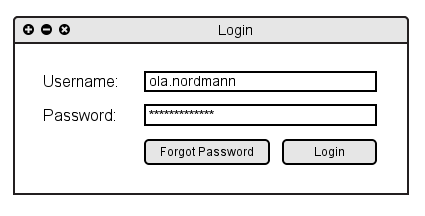
\includegraphics[scale=0.65]{images/login.png}
\caption{Loginvindu}
\label{login_image}
\end{figure}

\subsubsection{Hovedvindu}
Hovedvinduet har oversikten over avtalene i en uke-visning og en liste over notifikasjonene som berører brukeren (avtaler som har blitt endret eller kansellert). Forskjellige visninger som arbeidsdager, enkle dager, månedvisningen samt klokkeslett på venstresiden er ikke tatt med her. Det er tre forskjellige knapper, \emph{ny avtale}, \emph{flere kalendere} og \emph{logg ut}. \emph{Ny avtale} og \emph{flere kalendere} bringer opp nye vindu, mens \emph{logg ut} logger ut brukeren, lukker vinduet og bringer tilbake loginvinduet.

\begin{figure}[H]
\centering
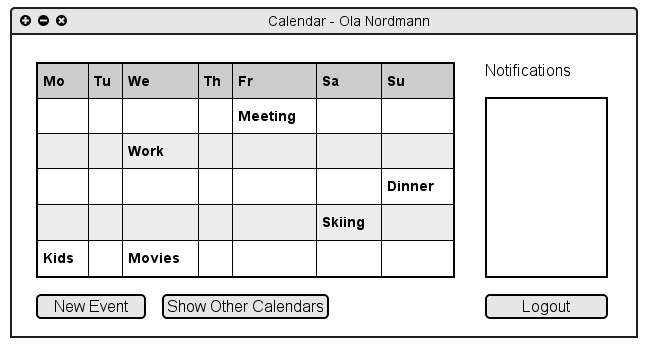
\includegraphics[scale=0.65]{images/hovedvindu.png}
\caption{Hovedvindu}
\label{hovedvindu_image}
\end{figure}

\subsubsection{Avtaleviser}
hello

\begin{figure}[H]
\centering
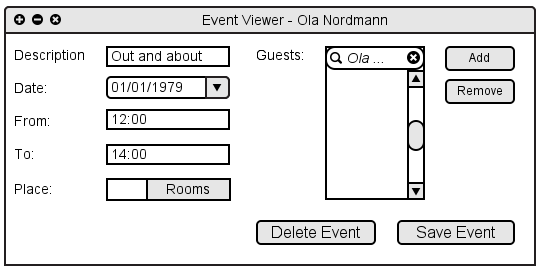
\includegraphics[scale=0.65]{images/avtaleviser.png}
\caption{Avtaleviser}
\label{avtaleviser_image}
\end{figure}

\subsubsection{Romreservasjon}
hello

\begin{figure}[H]
\centering
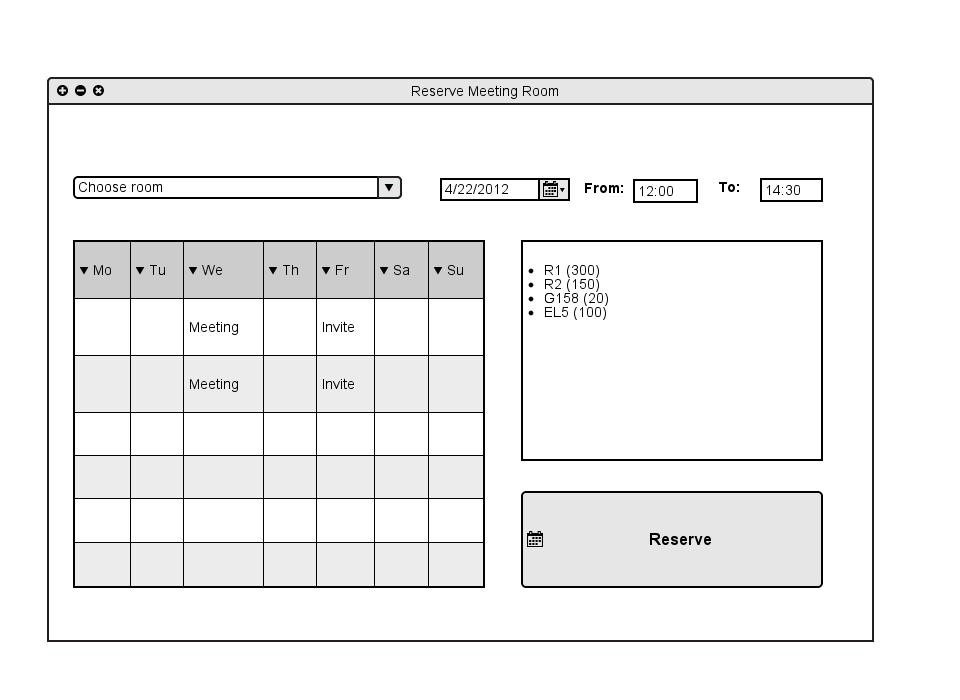
\includegraphics[scale=0.65]{images/romreservasjon.png}
\caption{Romreservasjon}
\label{romreservasjon_image}
\end{figure}

\subsubsection{Flere kalendere}
hello

\begin{figure}[H]
\centering
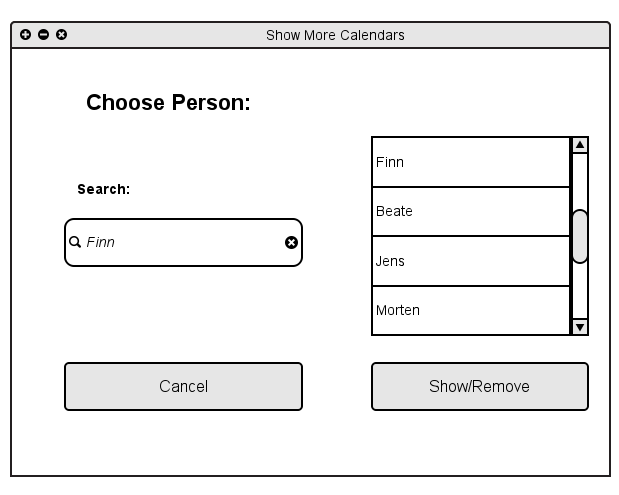
\includegraphics[scale=0.5]{images/flerekalendere.png}
\caption{Flerekalendere}
\label{flerekalendere_image}
\end{figure}

\subsubsection{Notifikasjon}
hello

\begin{figure}[H]
\centering
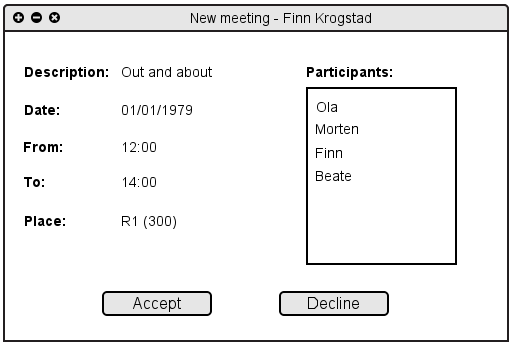
\includegraphics[scale=0.65]{images/notifikasjon_akseptert.png}
\caption{Notifikasjon akseptert}
\label{notifikasjon_akseptert_image}
\end{figure}

\begin{figure}[H]
\centering
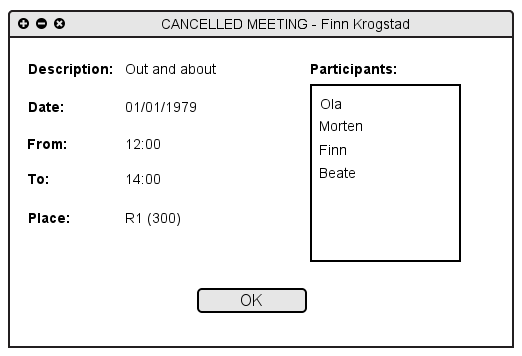
\includegraphics[scale=0.65]{images/notifikasjon_kanselert.png}
\caption{Notifikasjon kanselert}
\label{notifikasjon_kanselert_image}
\end{figure}


\subsection{Tilstandsdiagram}
Tilstandsdiagram

\begin{figure}[H]
\centering
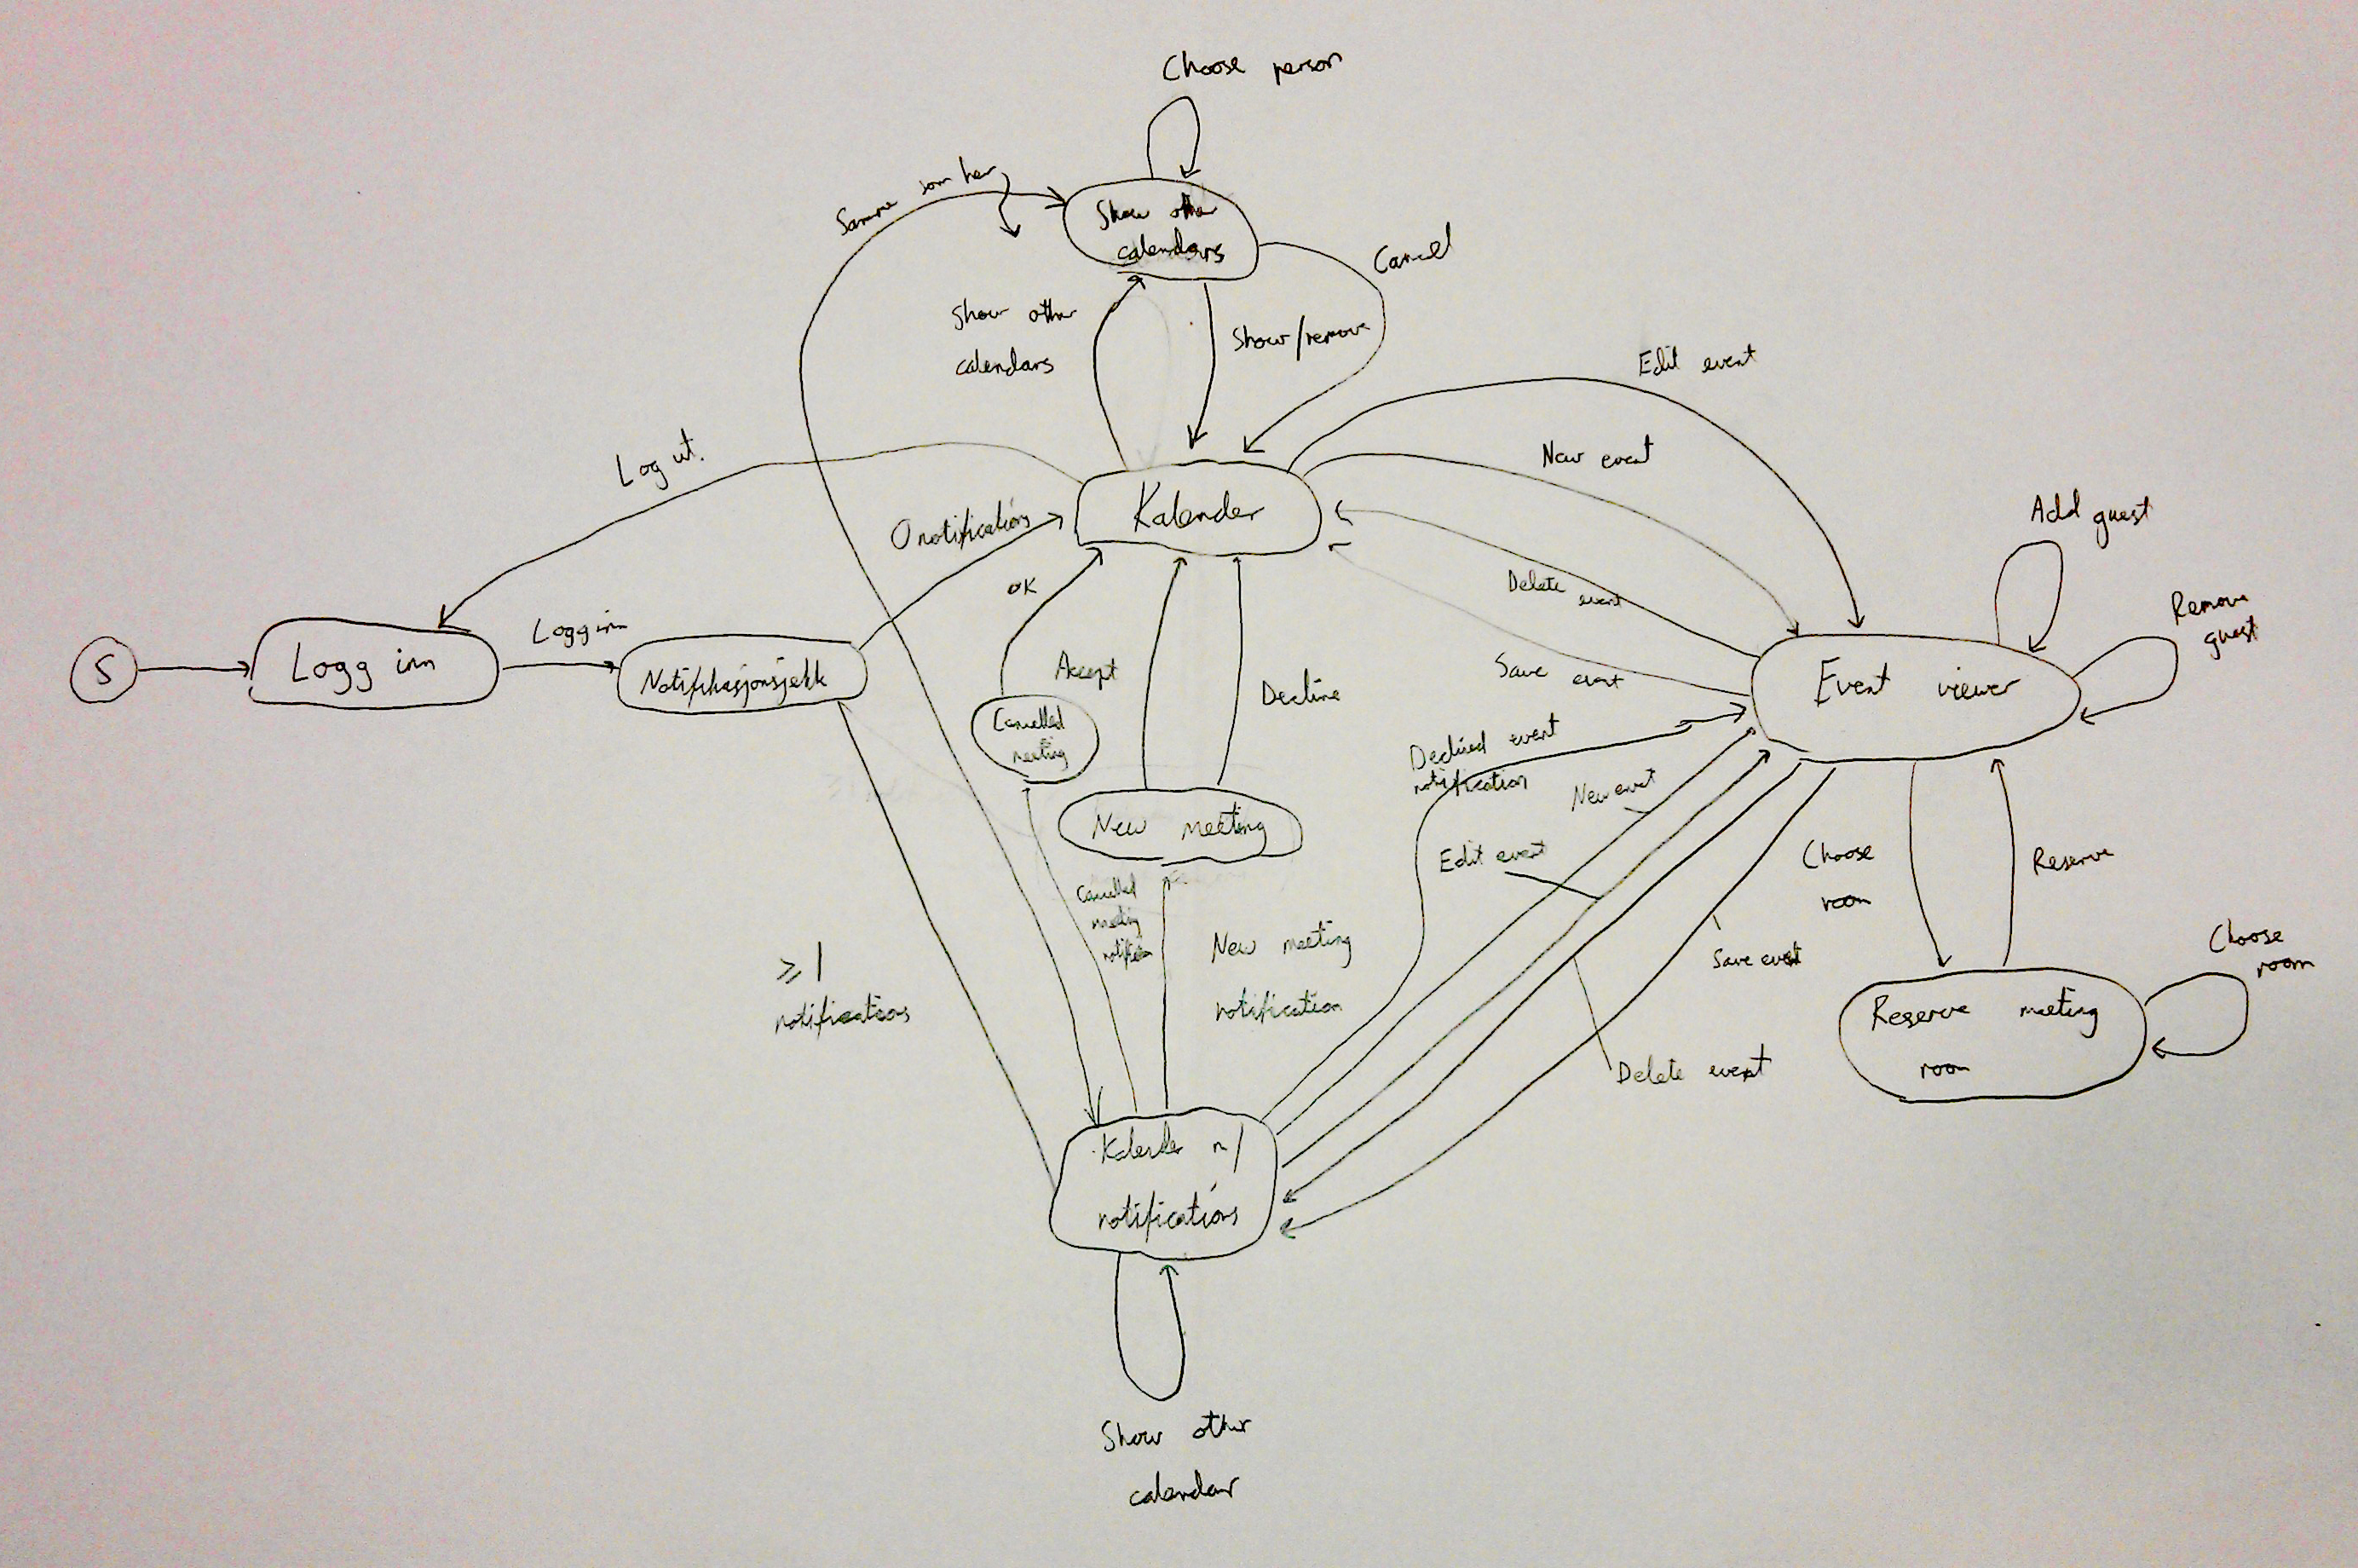
\includegraphics[scale=0.165]{images/tilstandsdiagram.jpg}
\caption{Tilstandsdiagram}
\label{tilstandsdiagram_image}
\end{figure}